\documentclass[linenumbers]{aastex631}

\usepackage{amsmath}

\shorttitle{Correcting K-correction}
\shortauthors{Evans}

\begin{document}

\title{Correcting K-correction: dark energy is based on a math error from 1930}

\correspondingauthor{Logan P. Evans}
\email{loganpevans@gmail.com}

\author[0000-0001-6450-3262]{Logan P. Evans}

\begin{abstract}
We rederive the K-correction equation and discover that the version of the
equation used to compute magnitudes contains three errors. The oldest of these
errors traces back nine decades; in 1930 the equation did not correct for
spectral bandwidth stretching, followed by a rederivation in 1968 that
accounted for spectral bandwidth stretching but did not correct for time
dilation. Two new errors were introduced in 1996, one of which causes
systematic distance biases by inverting the zero-point correction term. We
conclude that properly correcting apparent magnitudes for redshift resolves two
of the preeminent mysteries in cosmology: first, dark energy is not supported
by observations of Type Ia supernovae and second, the Hubble tension is due to
the errors in the K-correction equation.
\end{abstract}

%% https://astrothesaurus.org
\keywords{Type Ia supernovae(1728) --- Apparent magnitude(59)}

\section{Introduction}

The estimate of Type Ia supernovae (SnIa) distances is one of the primary
sources of data for cosmological models. Performing these distance estimates
involves taking a measurement of redshifted light in our observation frame and
then calculating the rest frame magnitude as if no redshift had occurred. It is
standard to report rest frame magnitudes in the $B$ filter, which is sensitive to
blue light, regardless of the filter used to take measurements in the
observation frame. The equation that converts from an observation frame
magnitude to a rest frame magnitude in the $B$ filter is called K-correction.

The first formal derivation of K-correction was performed by
\citet{tolman1930}, but it did not account for spectral bandwidth stretching,
one of the dimming effects of redshift. An alternative K-correction was
correctly derived by \citet{desitter1934}. However, in \citet{hubble1935}, the
discrepancy was noted yet dismissed. \citet{oke1968} rederived the K-correction
equation.  They accounted for spectral bandwidth stretching, but they did not
account for time dilation, one of the other dimming effects of redshift. The
paper by \citet{kim1996}, which is the basis for modern implementations of
K-correction, extended the work of \citet{oke1968} to handle additional
cross-filter comparisons and added a term that was intended to address
zero-point corrections. This history is explored in more depth in Section
\ref{sec:history}.

The effect of using an incorrect magnitude for SnIa is that we think objects
are farther away than they really are, and the effect compounds for greater
distances. Up until \citet{riess1998}, we did not have distant enough
observations for this error to matter much for cosmological models, but by the
late 1990s, it became clear that our measurements for distance and redshift were
not linear. This realization led to a model that utilized a cosmological
constant $\Lambda$ and dark energy in order to explain the non-linear
distance-redshift graph. We will show in Section \ref{sec:tension} that
correcting the flaw with K-correction leads to a linear graph that does not
need to rely on a cosmological constant.

\citet{planck2015} used an alternative technique to compute the Hubble constant
$H_0$ that is based on measurements of the cosmic microwave background (CMB).
CMB-based computations of $H_0$ has made it evident that something was missing
with our understanding of cosmology because this technique produces a
significantly different value than when the constant is derived using SnIa.  As
we will discuss in Section \ref{sec:tension}, fixing the error with
K-correction produces a measurement of the Hubble constant that is compatible
with models based on the CMB.

\section{A brief history of K-correction}
\label{sec:history}

Observational data from SnIa are essential for the calibration of models that
use redshift to estimate distance. The approximately linear relationship
between redshift and luminosity distance, often called the Hubble-Lema\^{i}tre law,
describes how quickly the universe is expanding. However, \citet{riess1998}
and \citet{perlmutter1999} presented evidence that there isn't a linear
relationship between redshift and distance, but instead, distant objects are
farther away than their redshift would predict (see Figure
\ref{fig:mu_distance_vs_redshift}). This phenomenon implies that the
acceleration of the universe is faster today than it was for old observations.
Previously the cause of this phenomenon was unknown and was referred to as dark
energy.

\begin{figure}
  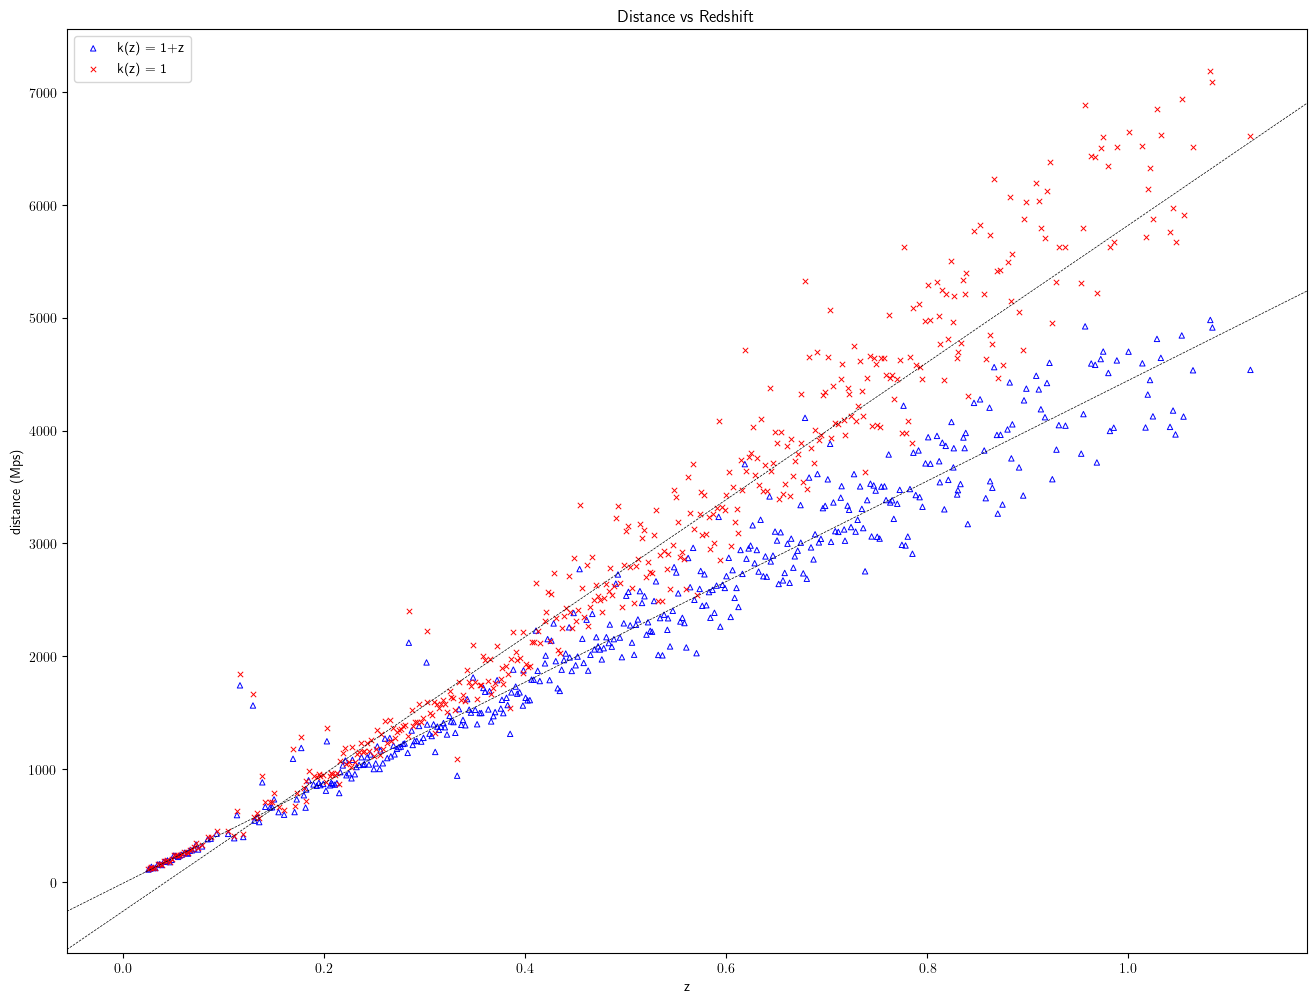
\includegraphics[width=\linewidth]{mu_distance_vs_redshift.png}
  \caption{The relationship between distance and redshift for two treatments of
  magnitude data. The displayed points are roughly a third of the values in the
  full SnIa dataset published in \citet{abbott2024}, selected evenly to aid
  visibility. The $k(z) = 1$ treatment, which represents the uncorrected
  values, is clearly non-linear while the $k(z) = 1 + z$ treatment which fixes
  the K-correction redshift error, appears to be linear.}
  \label{fig:mu_distance_vs_redshift}
\end{figure}

SnIa are used to explore the relationship between distance and redshift because
these events always happen in similar ways, which keeps the absolute brightness
roughly constant. An analogy is to imagine someone walking in the dark and
lighting matches. If we know how brightly a match burns at a known distance, we
can estimate the distance to any match by measuring the apparent brightness
before applying some geometry.

However, redshifting light dims an observation in three ways:

\begin{itemize}
  \item The energy of a wave is inversely proportional to its wavelength; thus a
  redshift of $z$ means the amount of energy per photon is reduced by a factor
  of $1 / (1+z)$.

  \item The bandwidth stretches. If a rest frame observes photons
  between the wavelengths of 400nm and 401nm, then a redshift of $z = 1$
  stretches the wavelength from 800nm to 802nm.

  \item Cosmological time dilation reduces the rate at which photons arrive.
\end{itemize}

To complicate matters, we use the $B$ band magnitude to calculate luminosity
distance. We want to know how bright a supernova appears for wavelengths around
445nm as if no redshift had occurred. However, we typically need to observe the
supernova with a filter that is sensitive to longer wavelengths, such as the
$i$ band filter which is sensitive to wavelengths from 700nm-850nm
\citep{flaugher2015}. The K-correction formula allows us to take a magnitude
measured in an observation filter $y$ and compute the magnitude in the target
filter $y$.

The first mathematical treatments of K-correction was performed by
\citet{tolman1930}. However, when Tolman made his derivation, he did not
consider the effects of a spectrum that is stretched due to redshift. See
the top two panels of Figure \ref{fig:k-example} for an example of this effect.

A few years later, \citet{desitter1934}, discussed all three issues that reduce
the observed magnitude of a distant observation. The correction for each of
these issues is identical: take a measurement for luminosity and multiply it by
the factor $1 + z$.

A year later, \citet{hubble1935} published a similar set of calculations for
K-correction, but these equations used $(1 + z)^2$ instead of the $(1 + z)^3$
correction term used by de Sitter. They started their derivation by copying the
incorrect equation from 1930. After their derivation, they noted:

\begin{quote}
It should be specially noted that this expression differs from the correction
to $m$ proposed by de Sitter, which contains the term $(1 + z)^3$ instead of
$(1 + z)^2$. Expression (28), however, would seem to give the proper correction
to use in connection with our equation (21), since it has been derived in such
a way as to make appropriate allowance, first, for the double effect of nebular
recession in reducing both the individual energy and the rate of arrival of
photons, and then for the further circumstance that a change in spectral
distribution of the energy that does arrive will lead to changes in its
photographic effectiveness.
\end{quote}

The Hubble K-correction with the incorrect correction term have been used ever
since.

By \citet{oke1968}, the two factors of $(1 + z)$ were attributed to the change
in energy and to the spectral bandwidth elongation, which leaves time dilation
as the factor that was omitted. A graph that demonstrates why it is essential to
correct for both the spectra bandwidth stretching and time dilation is presented
in Figure \ref{fig:k-example}.

\begin{figure}
  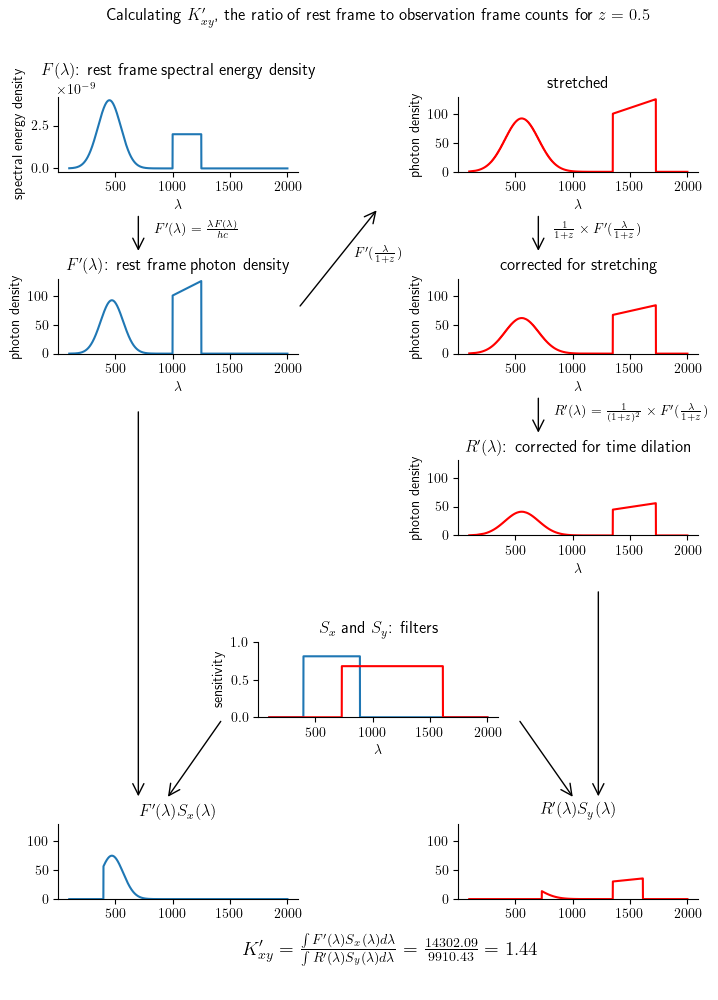
\includegraphics[width=.75\linewidth, height=0.75\vsize]{k_equation_flow.png}
  \caption{The ratio $K'_{xy}$ is the crux of the K-correction algorithm. We
  are able to observe a SnIa in the redshifted observation frame, but we want
  to compute the magnitude in the rest frame as if no redshift has occurred.
  This computation starts with $F(\lambda$, the spectral energy density that
  describes the expected luminosity in the rest frame. Using the SED, we can
  compute the photon density $F'(\lambda)$ for the rest frame. We show the
  process of computing $R'(\lambda$, the photon density in the observation
  frame, in three phases starting at the top right of the figure. First we
  stretch the photon density, but this step inflates counts. In the second
  step, we correct for the inflated counts by multiplying by $1/(1+z)$;
  at this point, the total count equals the total count of $F'(\lambda)$.
  Finally, in the third step we finish calculating the observation frame photon
  density $R'(\lambda)$ by accounting for time dilation, which also reduces
  photon counts by a factor of $1/(1+z)$.  Given the rest frame and
  observation frame photon densities, we can compute the expected ratio of
  photons by totalling the area under the curves in the two panels at the
  bottom of the graph. This example does not show the process of converting
  photon flux to magnitude, nor does it address the zero-point correction.
  }
  \label{fig:k-example}
\end{figure}

The modern treatment of K-correction is based on the work of \citet{kim1996}.
This work extended the calculations of K-correction to extend to filters beyond
the blue $B$ and visible $V$ bands. It also introduced a term that deals with
the zero-point for the actual filters. In the modern day, filters measure the
photon flux as opposed to the energy flux. Historically, bolometric devices
would measure the energy flux, but modern charge-coupled device (CCD) cameras
effectively measure the photon flux.

Quoting \citet{kim1996}:

\begin{quote}
  Therefore, the correct K correction calculation to be used with measured
  photometric magnitudes is the integral photon counts:

  \begin{equation}
  \label{eq:kim}
    K_{xy} =
      -2.5\text{log} \left(
        \frac{\int \lambda \mathcal{Z}(\lambda)S_x(\lambda)d\lambda}
             {\int \lambda \mathcal{Z}(\lambda)S_y(\lambda)d\lambda}\right)
      + 2.5\text{log}(1+z)
      + 2.5\text{log}\left(
        \frac{\int \lambda F(\lambda)S_x(\lambda)d\lambda}
             {\int \lambda F(\lambda/(1+z))S_y(\lambda))d\lambda}\right).
  \end{equation}
\end{quote}

This equation has three errors that we will explore in Section
\ref{sec:consequences}.

\section{Derivation of K-correction}
\label{sec:derivation}

With modern CCD cameras, a telescope observation consists of a single value
$\mathcal{F}_x$ erg/s, which represents the energy collected in filter $x$ per
second. A summary of how this works is provided by \citet{lesser2015}.
Photogenerated electrons are collected in potential wells, which means that the
measured energy is proportional to the number of photons. However, we need to
calculate the expected number of photons collected by using a spectral energy
density function $F$. The value $F(\lambda)$ gives the amount of energy
collected by a bolometric device for the wavelength $\lambda$.

To convert the spectral energy density $F$ to the photon density $F'$, we need
to use the Plank relation $E = hc / \lambda$ where $E$ is the energy, $h$
is Planck's constant, and $c$ is the speed of light. This gives us

\begin{equation}
\begin{aligned}
   F(\lambda) &= F'(\lambda) \times \frac{hc}{\lambda} \\
  F'(\lambda) &= \frac{\lambda F(\lambda)}{hc}.
\end{aligned}
\end{equation}

It is important to note that for the blueshifted wavelength $\lambda / (1+z)$,
this equation produces

\begin{equation}
 F'\left(\frac{\lambda}{1+z}\right) = \frac{\lambda}{(1+z)hc} F\left(\frac{\lambda}{1+z}\right).
\end{equation}

However, this equation is misleading and error prone. We will want to use it to
help calculate the amount of flux in an observation filter at the redshifted
wavelength $\lambda \times (1 + z)$. In other words, we want to produce the
photon density function $R'$ that is the redshifted version of $F'$.
Redshifting the photon density does two things:

\begin{itemize}
  \item The stretching of space increases the distance between photons while
  they are traveling. This phenomenon appears to an observer like time
  dilation, although cosmological time dilation is due to a different mechanism
  than relativistic time dilation. This effect reduces the photon arrival rate
  by a factor of $1/(1+z)$.

  In order to account for cosmological time dilation, we will need to multiply
  $F'$ by $1/(1+z)$.

  \item All wavelengths are changed by a factor of $1 + z$. When we integrate
  $R'$ from wavelength $\lambda_a$ to wavelength $\lambda_b$, the values
  correspond to the wavelengths $\lambda_a / (1+z)$ to $\lambda_b / (1+z)$ in
  $F'$. We will integrate over a width of $\lambda_b - \lambda_a$, but
  $F'(\lambda / (1+z))$ will refer to values in a width of
  $(\lambda_b - \lambda_a) / (1+z)$.

  In order to account for this spectral bandwidth stretching effect, we will need
  to multiply $F'$ by a second factor of $1/(1+z)$.
\end{itemize}

Combining these two phenomena, we can calculate the redshifted spectral energy
density $R$ using

\begin{equation}
\begin{aligned}
\label{eq:redshifted_density}
  R'(\lambda) &= F'\left(\frac{\lambda}{1+z}\right) \times \frac{1}{(1 + z)^2} \\
  R(\lambda) &= \frac{\lambda}{(1+z)hc} \times F\left(\frac{\lambda}{1+z}\right) \times \frac{1}{(1 + z)^2} .
\end{aligned}
\end{equation}

We deliberately do not combine all of the factors of $1+z$ together because
this form is more natural to implement in code.

In order to calculate the amount of flux $\mathcal{F}_x$ measured in filter
$x$, we need to compute the photon density $F'(\lambda)$ and multiply it by
sensitivity $S_x(\lambda)$, which represents the proportion of photons filter $x$
will measure at wavelength $\lambda$. We then need to sum over all wavelengths,
which is expressed with the equation

\begin{equation}
\begin{aligned}
\label{eq:flux_definition}
  \mathcal{F}_x &= \int F'(\lambda) S_x(\lambda) d\lambda \\
                &= \int \lambda F(\lambda) S_x(\lambda) d\lambda.
\end{aligned}
\end{equation}

The limits of integration are technically from 0 to $\infty$, but these are
usually not written because the sensitivity $S(\lambda)$ is 0 for wavelengths
outside of a filter's bandpass.

We will also use the energy flux $\mathcal{F}$ to magnitude $m$ formula:

\begin{equation}
\begin{aligned}
\label{eq:flux2mag}
                             m_x &= -2.5 \text{log}(\mathcal{F}_x) + P_x \\
  -2.5 \text{log}(\mathcal{F}_x) &= m_x - P_x .
\end{aligned}
\end{equation}

$P_x$ represents the zero-point for the filter $x$ on some particular
telescope. In order to use consistent magnitude values across telescopes that
have different light gathering abilities, we take the measured magnitude and
multiply it by the ratio of the standard flux rate to the flux rate for this
particular telescope and filter. For convenience, we use $P_x = -2.5
\text{log}(P'_x)$ so that we can work with flux instead of with magnitude.

Now that we have the identities in Equations \ref{eq:flux_definition} and
\ref{eq:flux2mag} we will change directions and look at the definition of
K-correction $K_{xy}$. This value allows us to make an observation in filter
$y$ and report what the magnitude would have been in filter $x$ if no redshift
occurred:

\begin{equation}
\begin{aligned}
\label{eq:definition}
  m_y &= M_x + \mu + K_{xy} \\
      &= M_x + m_x - M_x + K_{xy} \\
      &= m_x + K_{xy} \\
  m_x &= m_y - K_{xy} .
\end{aligned}
\end{equation}

\noindent The second line of Equation \ref{eq:definition} expands the distance modulus
$\mu$ using $\mu = m - M$ where $m$ is the observed magnitude and $M$ is the
absolute magnitude.

Since the K-correction is a magnitude value and we wish to work on flux values,
it is convenient to define the following substitution:

\begin{equation}
\label{eq:k_substitution}
  K_{xy} = 2.5\text{log}(K'_{xy}) .
\end{equation}

Note that this substitution omits the minus ($-$) sign that we used on a
similar substitution for $P_x$.

Starting with Equation \ref{eq:flux2mag} and then
recombining the flux term $\mathcal{F}_y$ with $m_y$ from Equation
\ref{eq:definition}, we have

\begin{equation}
\begin{aligned}
\label{eq:as_flux}
  -2.5 \text{log}(\mathcal{F}_x)
      &= m_x - P_x \\
      &= m_y - K_{xy} - P_x \\
      &= -2.5 \text{log}(\mathcal{F}_y) + P_y - K_{xy} - P_x \\
      &= -2.5 \text{log}(\mathcal{F}_y)
         - 2.5 \text{log}(P'_y)
         - 2.5 \text{log}(K'_{xy})
         + 2.5 \text{log}(P_x) \\
      &= -2.5 \left(
         \text{log}(\mathcal{F}_y)
         + \text{log}(K'_{xy})
         + \text{log}(P'_y)
         - \text{log}(P'_x)
        \right) \\
      &= -2.5 \text{log}\left(
        \mathcal{F}_y
        \times K'_{xy}
        \times \frac{P'_y}{P'_x}\right) \\
  \mathcal{F}_x &= \mathcal{F}_y \times K'_{xy} \times \frac{P'_y}{P'_x}.
\end{aligned}
\end{equation}

It is useful to consider whether the term $P'_y / P'_x$ is correct or if
it should be inverted, but if we rewrite Equation \ref{eq:as_flux} as

\begin{equation}
  \mathcal{F}_x \times P'_x = \mathcal{F}_y \times P'_y \times K'_{xy}
\end{equation}

\noindent then the meaning becomes more clear. The left side, $\mathcal{F}_x
\times P'_x$, is the rate of photon collection for an idealized telescope in
filter $x$ while $\mathcal{F}_y \times P'_y$ is the rate of photon collection
for an idealized telescope in filter $y$. We observe the value $\mathcal{F}_y
\times P'_y$ and want to use the fudge factor $K'_{xy}$ to produce the value
$\mathcal{F}_x \times P'_x$.

We can isolate $K'_{xy}$ and then use Equation \ref{eq:flux_definition} to expand

\begin{equation}
\begin{aligned}
  \mathcal{F}_x &= \mathcal{F}_y \times K'_{xy} \times \frac{P'_y}{P'_x} \\
        K'_{xy} &= \frac{P'_x}{P'_y} \times \frac{\mathcal{F}_x}{\mathcal{F}_y} .
\end{aligned}
\end{equation}

We now use Equations \ref{eq:redshifted_density} and \ref{eq:flux_definition}
to calculate the fluxes $\mathcal{F}_x$ and $\mathcal{F}_y$ in terms of the
spectral energy density function $F$. Note that $\mathcal{F}_x$ uses the rest
frame spectral energy density $F$, while $\mathcal{F}_y$ uses the redshifted
spectral energy density $R(\lambda)$:

\begin{equation}
\begin{aligned}
  K'_{xy} &= \frac{P'_x}{P'_y} \times \frac{\mathcal{F}_x}{\mathcal{F}_y} \\
         &= \frac{P'_x}{P'_y} \times
              \frac{\int F'(\lambda) S_x(\lambda) d\lambda}
                   {\int R'(\lambda) S_y(\lambda) d\lambda} \\
         &= \frac{P'_x}{P'_y} \times
              \frac{\int F'(\lambda) S_x(\lambda) d\lambda}
                   {\int F'(\lambda / (1+z)) \times (1 / (1 + z)^2) S_y(\lambda) d\lambda} \\
         &= \frac{P'_x}{P'_y} \times (1+z)^2 \times
              \frac{\int (\lambda / hc) F(\lambda) S_x(\lambda) d\lambda}
                   {\int (\lambda / ((1+z)hc)) F(\lambda / (1+z)) S_y(\lambda) d\lambda} \\
         &= \frac{P'_x}{P'_y} \times (1 + z)^2 \times
              \frac{\int \lambda F(\lambda) S_x(\lambda) d\lambda}
                   {\int (\lambda / (1+z) F(\lambda / (1+z)) S_y(\lambda) d\lambda} .
\end{aligned}
\end{equation}

Finally, we can use Equation \ref{eq:k_substitution} to convert the flux $K'_{xy}$ back
into the magnitude $K_{xy}$:

\begin{equation}
\begin{aligned}
\label{eq:K2k}
  K_{xy} &= 2.5\text{log}(K'_{xy}) \\
         &= 2.5\text{log}\left(
            \frac{P'_x}{P'_y} \times (1 + z)^2 \times
            \frac{\int \lambda F(\lambda) S_x(\lambda) d\lambda}
                 {\int (\lambda / (1+z)) F(\lambda / (1+z)) S_y(\lambda) d\lambda}\right) \\
         &= 2.5 \left(
            \text{log} \left( \frac{P'_x}{P'_y} \right)
            + \text{log}( {(1 + z)^2})
            + \text{log}\left( \frac{\int \lambda F(\lambda) S_x(\lambda) d\lambda}
                                    {\int (\lambda / (1+z)) F((\lambda)/ (1+z)) S_y(\lambda) d\lambda}
            \right) \right) \\
         &= 2.5 \text{log} \left( \frac{P'_x}{P'_y} \right)
            + 5 \text{log} (1 + z)
            + 2.5 \text{log} \left(
              \frac{\int \lambda F(\lambda) S_x(\lambda) d\lambda}
                   {\int (\lambda / (1+z)) F(\lambda / (1+z)) S_y(\lambda) d\lambda} \right) \\
         &= 5 \text{log} (1 + z)
            + 2.5 \text{log} \left(
              \frac{\int \lambda F(\lambda) S_x(\lambda) d\lambda}
                   {\int (\lambda / (1+z)) F(\lambda / (1+z)) S_y(\lambda) d\lambda} \right)
            - P_x + P_y .
\end{aligned}
\end{equation}

\section{Consequences}
\label{sec:consequences}

In order to fully compare our derivation against Equation \ref{eq:kim}, we need
to use the identity

\begin{equation}
  P = -2.5 \text{log} \left( \int \frac{\lambda}{hc} \mathcal{Z}(\lambda) S(\lambda) d\lambda \right)
\end{equation}

\noindent where, according to \citet{kim1996}, ``$\mathcal{Z}(\lambda)$ is an
idealized spectral energy distribution at $z = 0$ for which
$U = B = V = R = I = 0$ in the photometric system being used.'' Combining this
with Equation \ref{eq:K2k}, we have

\begin{equation}
\begin{aligned}
  K_{xy} &= 5 \text{log} (1 + z)
            + 2.5 \text{log} \left(
              \frac{\int \lambda F(\lambda) S_x(\lambda) d\lambda}
                   {\int (\lambda / (1+z)) F(\lambda / (1+z)) S_y(\lambda) d\lambda} \right)
            - P_x + P_y \\
         &= 5 \text{log} (1 + z)
            + 2.5 \text{log} \left(
              \frac{\int \lambda F(\lambda) S_x(\lambda) d\lambda}
                   {\int (\lambda / (1+z)) F(\lambda / (1+z)) S_y(\lambda) d\lambda} \right) \\ &\ 
            + 2.5 \text{log} \left( \int (\lambda / hc) \mathcal{Z}(\lambda) S_x(\lambda) d\lambda \right)
            - 2.5 \text{log} \left( \int (\lambda / hc) \mathcal{Z}(\lambda) S_y(\lambda) d\lambda \right) \\
         &= 2.5 \text{log} \left(
              \frac{\int \lambda \mathcal{Z}(\lambda) S_x(\lambda) d\lambda}
                   {\int \lambda \mathcal{Z}(\lambda) S_y(\lambda) d\lambda}
             \right)
            + 5 \text{log} (1 + z)
            + 2.5 \text{log} \left(
              \frac{\int \lambda F(\lambda) S_x(\lambda) d\lambda}
                   {\int (\lambda / (1+z)) F(\lambda / (1+z)) S_y(\lambda) d\lambda} \right) .
\end{aligned}
\end{equation}

Three differences with Equation \ref{eq:kim} stand out:

\begin{itemize}
  \item The sign is different for the first term. This will have a subtle but
  frustrating effect for real measurements. The zero-point values are usually,
  but not always, close to zero. As we observe more distant supernovae, it is
  useful to switch our observational filter to a filter that is sensitive to
  longer wavelengths. Each observation filter will have its own small bias.

  This effect by itself can alter estimates of $H_0$ by several km s$^{-1}$
  Mpc$^{-1}$.  While we present an estimate of the Hubble constant in Figure
  \ref{fig:H0bootstrap}, we are not terribly confident in the numbers because
  we were unable to correct for the zero-point errors, or verify that these
  errors may not exist.

  \item The second term is multiplied by $2.5$ in \citet{kim1996}, but is
  multiplied by $5$ here. This is the manifestation of the error in
  \citet{tolman1930}.

  \item In our derivation, the third term has an extra $1 + z$ expression.
  Based on an inspection of the SN(oo)py software package presented by
  \citet{snpy}, this error is ignored and software package authors implement it
  as intended, not precisely as written.
\end{itemize}

\section{Dark energy and the Hubble tension}
\label{sec:tension}

As shown in Figure \ref{fig:mu_distance_vs_redshift}, when reported magnitudes
are corrected by adding the magnitude $-2.5\text{log}(1+z)$, there is a linear
relationship between redshift and luminosity distance. This is in accordance
with the Hubble-Lema\^{i}tre law. As opposed to the uncorrected values, there
is no visual acceleration.

Since the corrected values are approximately linear, we can use them to
estimate the Hubble constant $H_0$. This is demonstrated in Figure
\ref{fig:expansion}. Furthermore, we performed a bootstrap calculation to
estimate the distribution of $H_0$ estimates in Figure \ref{fig:H0bootstrap}.

The value estimated here, $H_0 \sim 65.94 \pm 1.29$ is highly suspicious
because of the flipped zero-point corrections, but it is consistent with
estimates of $H_0$ that are based on the CMB. \citet{planck2020} published the
CMB value of $H_0 \sim 67.27 \pm 0.6$, and the one sigma error bars overlap. It
is interesting to note that restricting the Dark Energy Survey observations of
SnIa \citep{vincenzi2024} to only those with $z < 0.1$, which presumably is a
small enough redshift that all observations will have been made with the same
filter, gives the estimate $H_0 \sim 67.8 \pm 1.86$.

\begin{figure}
  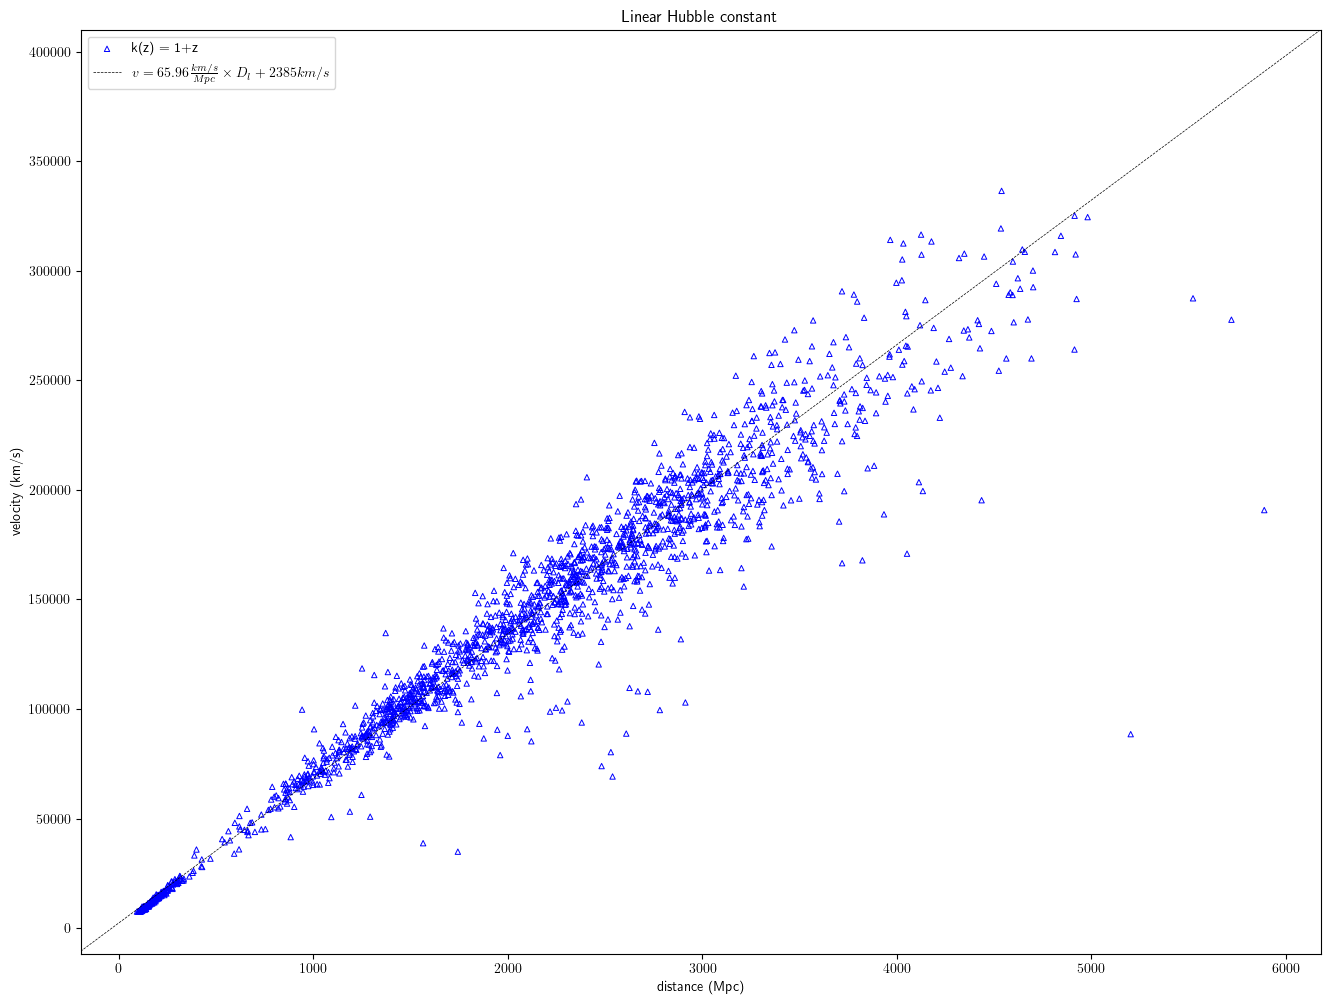
\includegraphics[width=\linewidth]{velocity_vs_distance.png}
  \caption{The relationship between expansion velocity and distance. The slope of this graph demonstrates the Hubble constant.
  }
\label{fig:expansion}
\end{figure}

\begin{figure}
  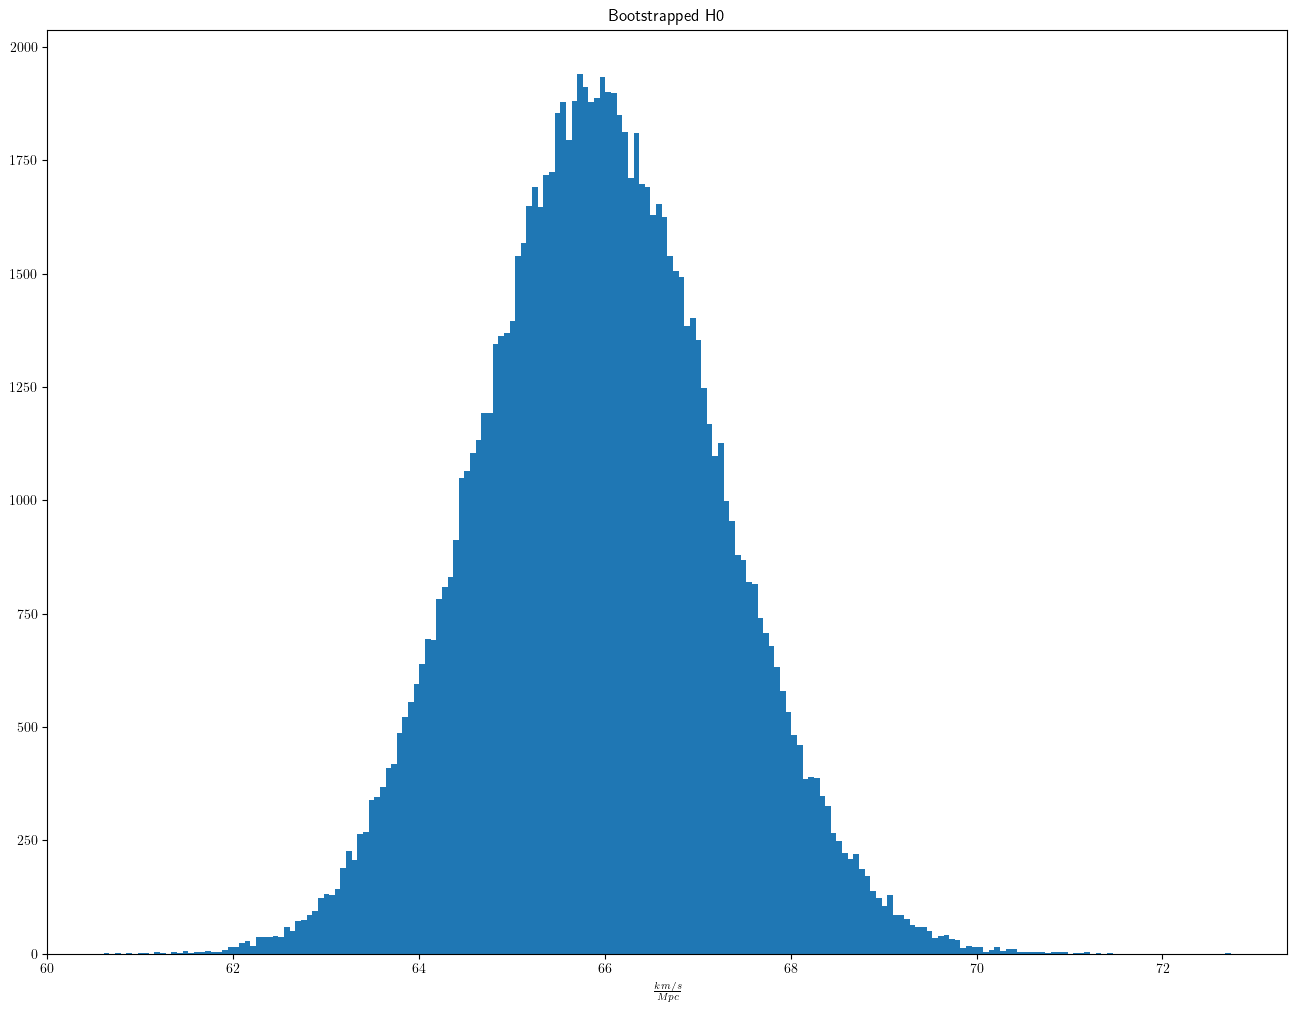
\includegraphics[width=\linewidth]{bootstrapped_H0.png}
  \caption{A histogram of $100{\small,}000$ bootstrap trials measuring the Hubble constant
  $H_0$. Each trial samples an absolute magnitude $M \sim Norm(-19.2334,
  0.0404)$ for SnIa based on data published by \citet{camarena2020}. It then samples,
  with replacement, a population of supernovae from the dataset published by
  \citet{abbott2024}. Finally, it uses the non-parametric linear regression
  technique described by \citet{siegel1982}. The result of the bootstrap is $H_0
  \sim Norm(65.94, 1.29^2)$.
  }
\label{fig:H0bootstrap}
\end{figure}

\section{Conclusions}

Since the K-correction error has corrupted all astronomical measurements that
depend on both magnitude and redshift, a lot of data needs to be reanalysed.
Cosmological parameters, such as those used by the
Friedmann-Lema\^{i}tre-Robertson-Walker (FLRW) metric or the $\Lambda$-CDM
model, can only be recalculated once the data is cleaned.

The reasons that the K-correction errors went undiscovered for so long should
also be explored. Many hints existed that something was wrong, yet the
problems persisted.

\bibliography{references}{}
\bibliographystyle{aasjournal}

\end{document}
